\section{Pattern recognition and track fitting approaches}

\subsection{Introduction to associative memory approach}

\subsubsection{From pattern recognition to track fitting}

\noindent Using associative memories in order to perform a fast pattern recognition (PR) at the trigger stage was first exposed in Ref.~\cite{bib:Del-89}. The principle is sketched in Fig.~\ref{fig:AM_principle}:
\begin{figure}[ht!]
\centering
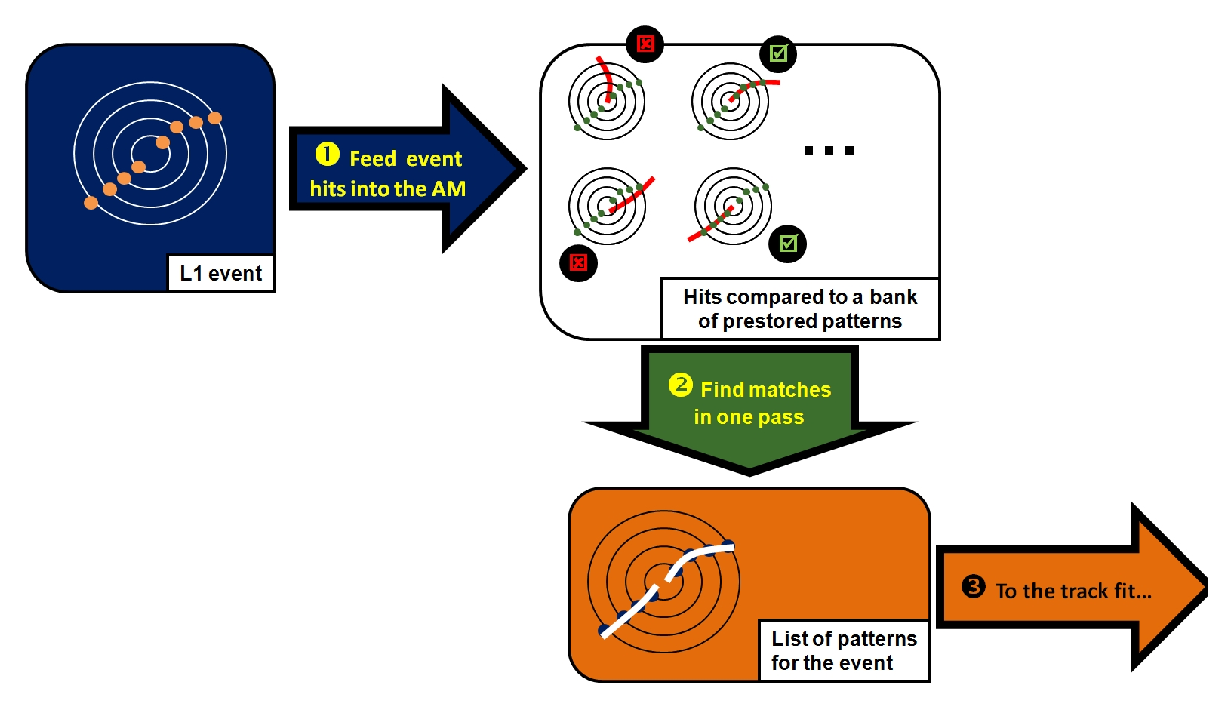
\includegraphics[width=0.7\columnwidth]{Plots/TriggerAM.eps}
\caption{Pattern recognition using associative memories.}
\label{fig:AM_principle}
\end{figure}

\noindent The idea is to compare the hits recorded in the tracking system to a bank of patterns stored in an associative memory chip. The patterns could be seen as low-granularity tracks, they are defined once for all using Monte-Carlo events, and they are ideally covering all the possible tracks occuring in the detector. In this part we will concentrate ourselves on the pattern bank definition. This is indeed the central point of the PR stage. The bank, which is defined using simulated events, has to fulfill few requirements. Before presenting them, it's important to define some parameters. 

\noindent A pattern can be defined as a road in the sector. Each road may contain one or more tracks, as shown on the Fig.~\ref{fig:pattern}. 
\begin{figure}[ht!]
\centering
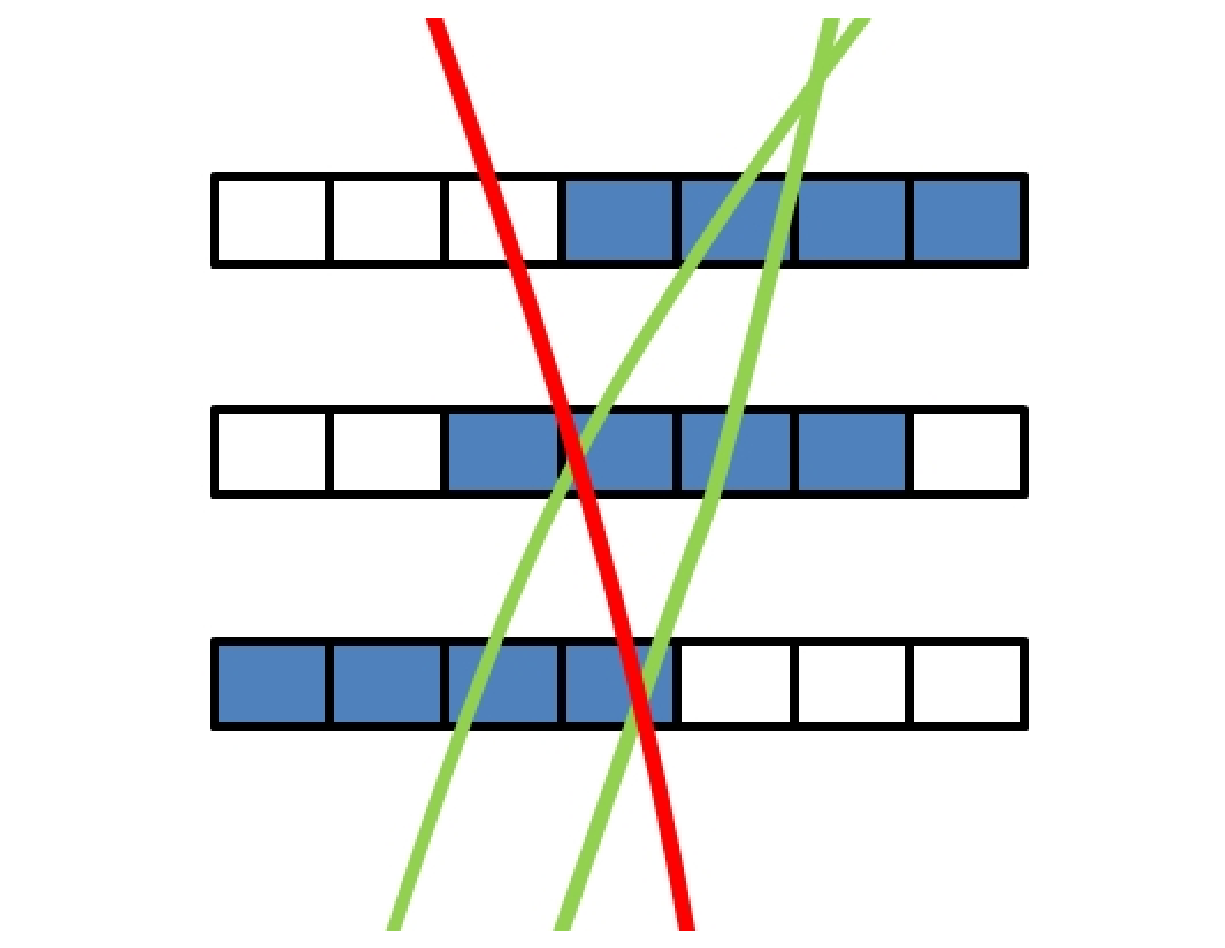
\includegraphics[width=0.3\columnwidth]{Plots/Pattern.eps}
\caption{A pattern in a three-layers detector. Green tracks will match the pattern, red tracks won't.}
\label{fig:pattern}
\end{figure}

\noindent On this picture one also get an idea of the pattern structure. Each pattern is made of one superstrip per layer. A superstrip is a group of strips/pixels, and is therefore heavily constrained by the detector itself. Once the superstrip definition has been set, its position information is coded in a N-bits word: the superstrip address. It is important to realize that the AM-based pattern recognition is using these addresses, and is therefore completely independent from the detector geometry.

\noindent As the addresses are transmitted to the AM independently for each layer, layer number doesn't have to be in the address word. In order to understand the address definition, Fig.~\ref{fig:sstrip_def} shows how a superstrip is defined in the barrel part of the tracker.  
\begin{figure}[ht!]
\centering
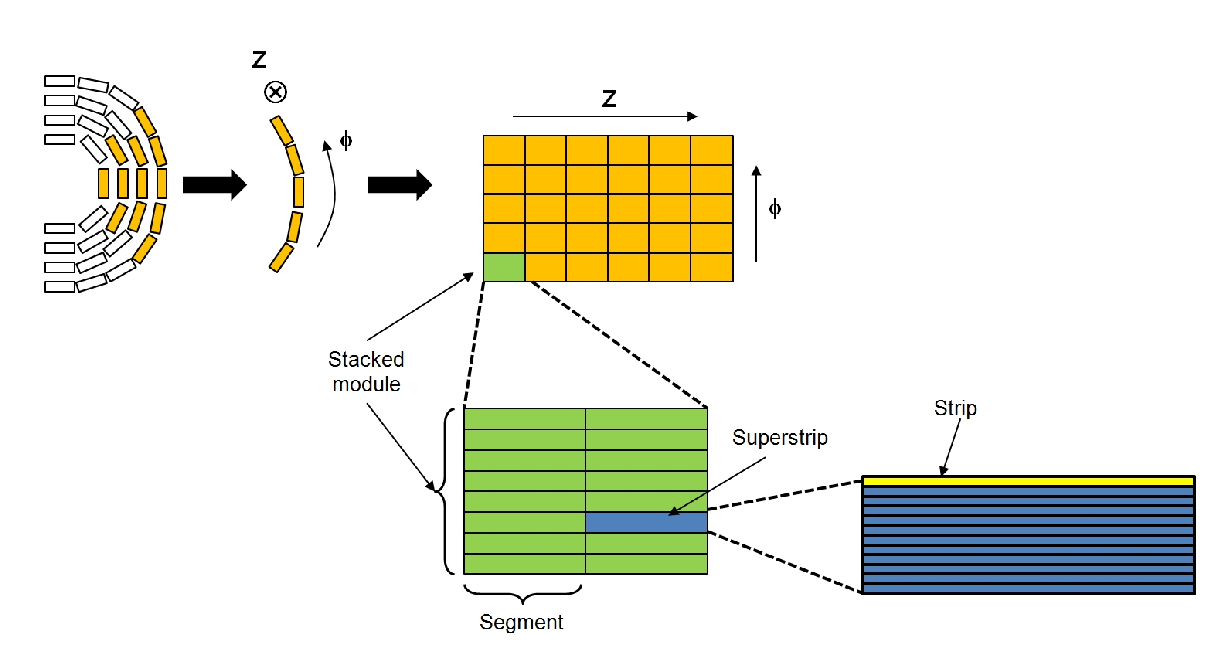
\includegraphics[width=0.7\columnwidth]{Plots/SStripDef.eps}
\caption{Geometric definition of a superstrip (barrel example).}
\label{fig:sstrip_def}
\end{figure}
\begin{figure}[ht!]
\centering
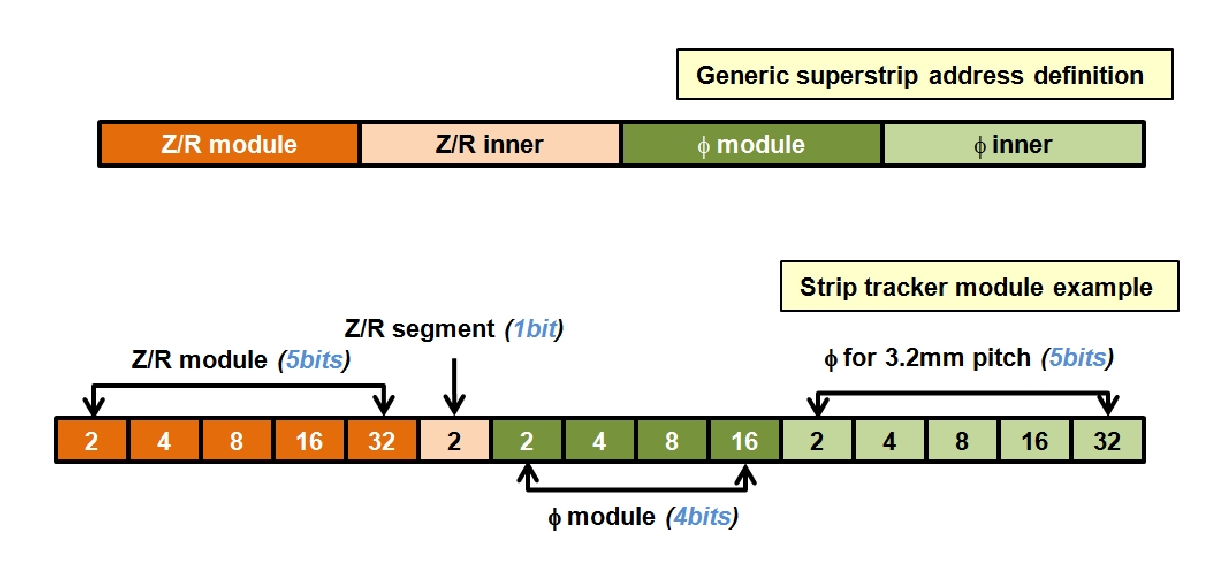
\includegraphics[width=0.7\columnwidth]{Plots/SSaddress.eps}
\caption{Address definition of a superstrip.}
\label{fig:SS_code}
\end{figure}

\noindent One has to be able to define a unique address to define the $z (resp. r)/\phi$ position of each superstrip in the barrel (resp. endcap) sector (r (resp. z) is given by the layer (resp. disk). The coding is sketched on Fig.~\ref{fig:SS_Code}. The number of bits necessary reflects the superstrip granularity and is constrained by the maximal word size acceptable by the AM chip (currently 16 bits). A first set of bits provides the module number along the corresponding coordinate: 5 bits for $Z$ (one could have up to 24 modules in Z in one sector) and 4 for $\phi$ (up to 11 modules per sector in the outermost layer). Then, for each coordinates, a second serie of bits provide the superstrip position within the module. Fig.~\ref{fig:sstrip_def} shows a tracker strip module (in green), divided into 2 segments in $Z$ and 1024 strip in $\phi$. Therefore in order to describe all the position, one would need only 1 bit for $Z$, and 10 bits for $\phi$. In practice, a certain number of strips are grouped to form the superstrip, in our case 32, thus leading to 5 in the address.   

\noindent For the endcap the coding is the same. z is just replaced by r (equivalence is made between disks and layers, ladders and rings). 

\subsection{System configuration}

\subsubsection{Trigger sectors definition}


\noindent The trigger definition is driven by two concurent constraints. As we will see later, the number of patterns will strongly depend on the sector size itself. It is therefore tempting to divide the detector into very small sectors, in order to work with small, easier to handle, banks. On the other hand, however, the minimal sector size will be geometrically constrained by the track trigger requirements. The system should indeed be able to detect tracks over a given $p_T$ threshold. The minimal sector should thus be able to entirely contain such tracks. For example, with a threshold of $2~GeV/c$, the minimal sector size is approximatively $18^{o}$.

\noindent This value sets the minimal overlap needed between two neghbouring sectors if one wants each track to be contained into at least one sector. In the following we divided the tracker into 8 sectors covering each $60^{o}$ in $\phi$, with therefore $20^{o}$ overlap between two consecutive sectors. The resulting division is shown on Fig.~\ref{fig:SEC_PHI}.


\subsubsection{Definition of the pattern banks used}



\clearpage
